\chapter{Sensoren}
\renewcommand{\kapitelautor}{Autor: Lucas Ullrich}

%%%%%%%%%%%%%%%%%%%%%%%%%%%%%%%%%%%%%%%%%%%%%%%%%%%%%%%%%%%%%%%%%%%%%%%%%%%%%%%
\section{Pixy CMUcam5}
Bei der PIXY CMUcam5 handelt es sich um ein Open Source Kameramodul, welches über eine Objekterkennung verfügt. Mit diesem ist es möglich sogenannte Colorcodes oder einfache Objekte zu erkennen.

\begin{figure}[H]
  \begin{centering}
    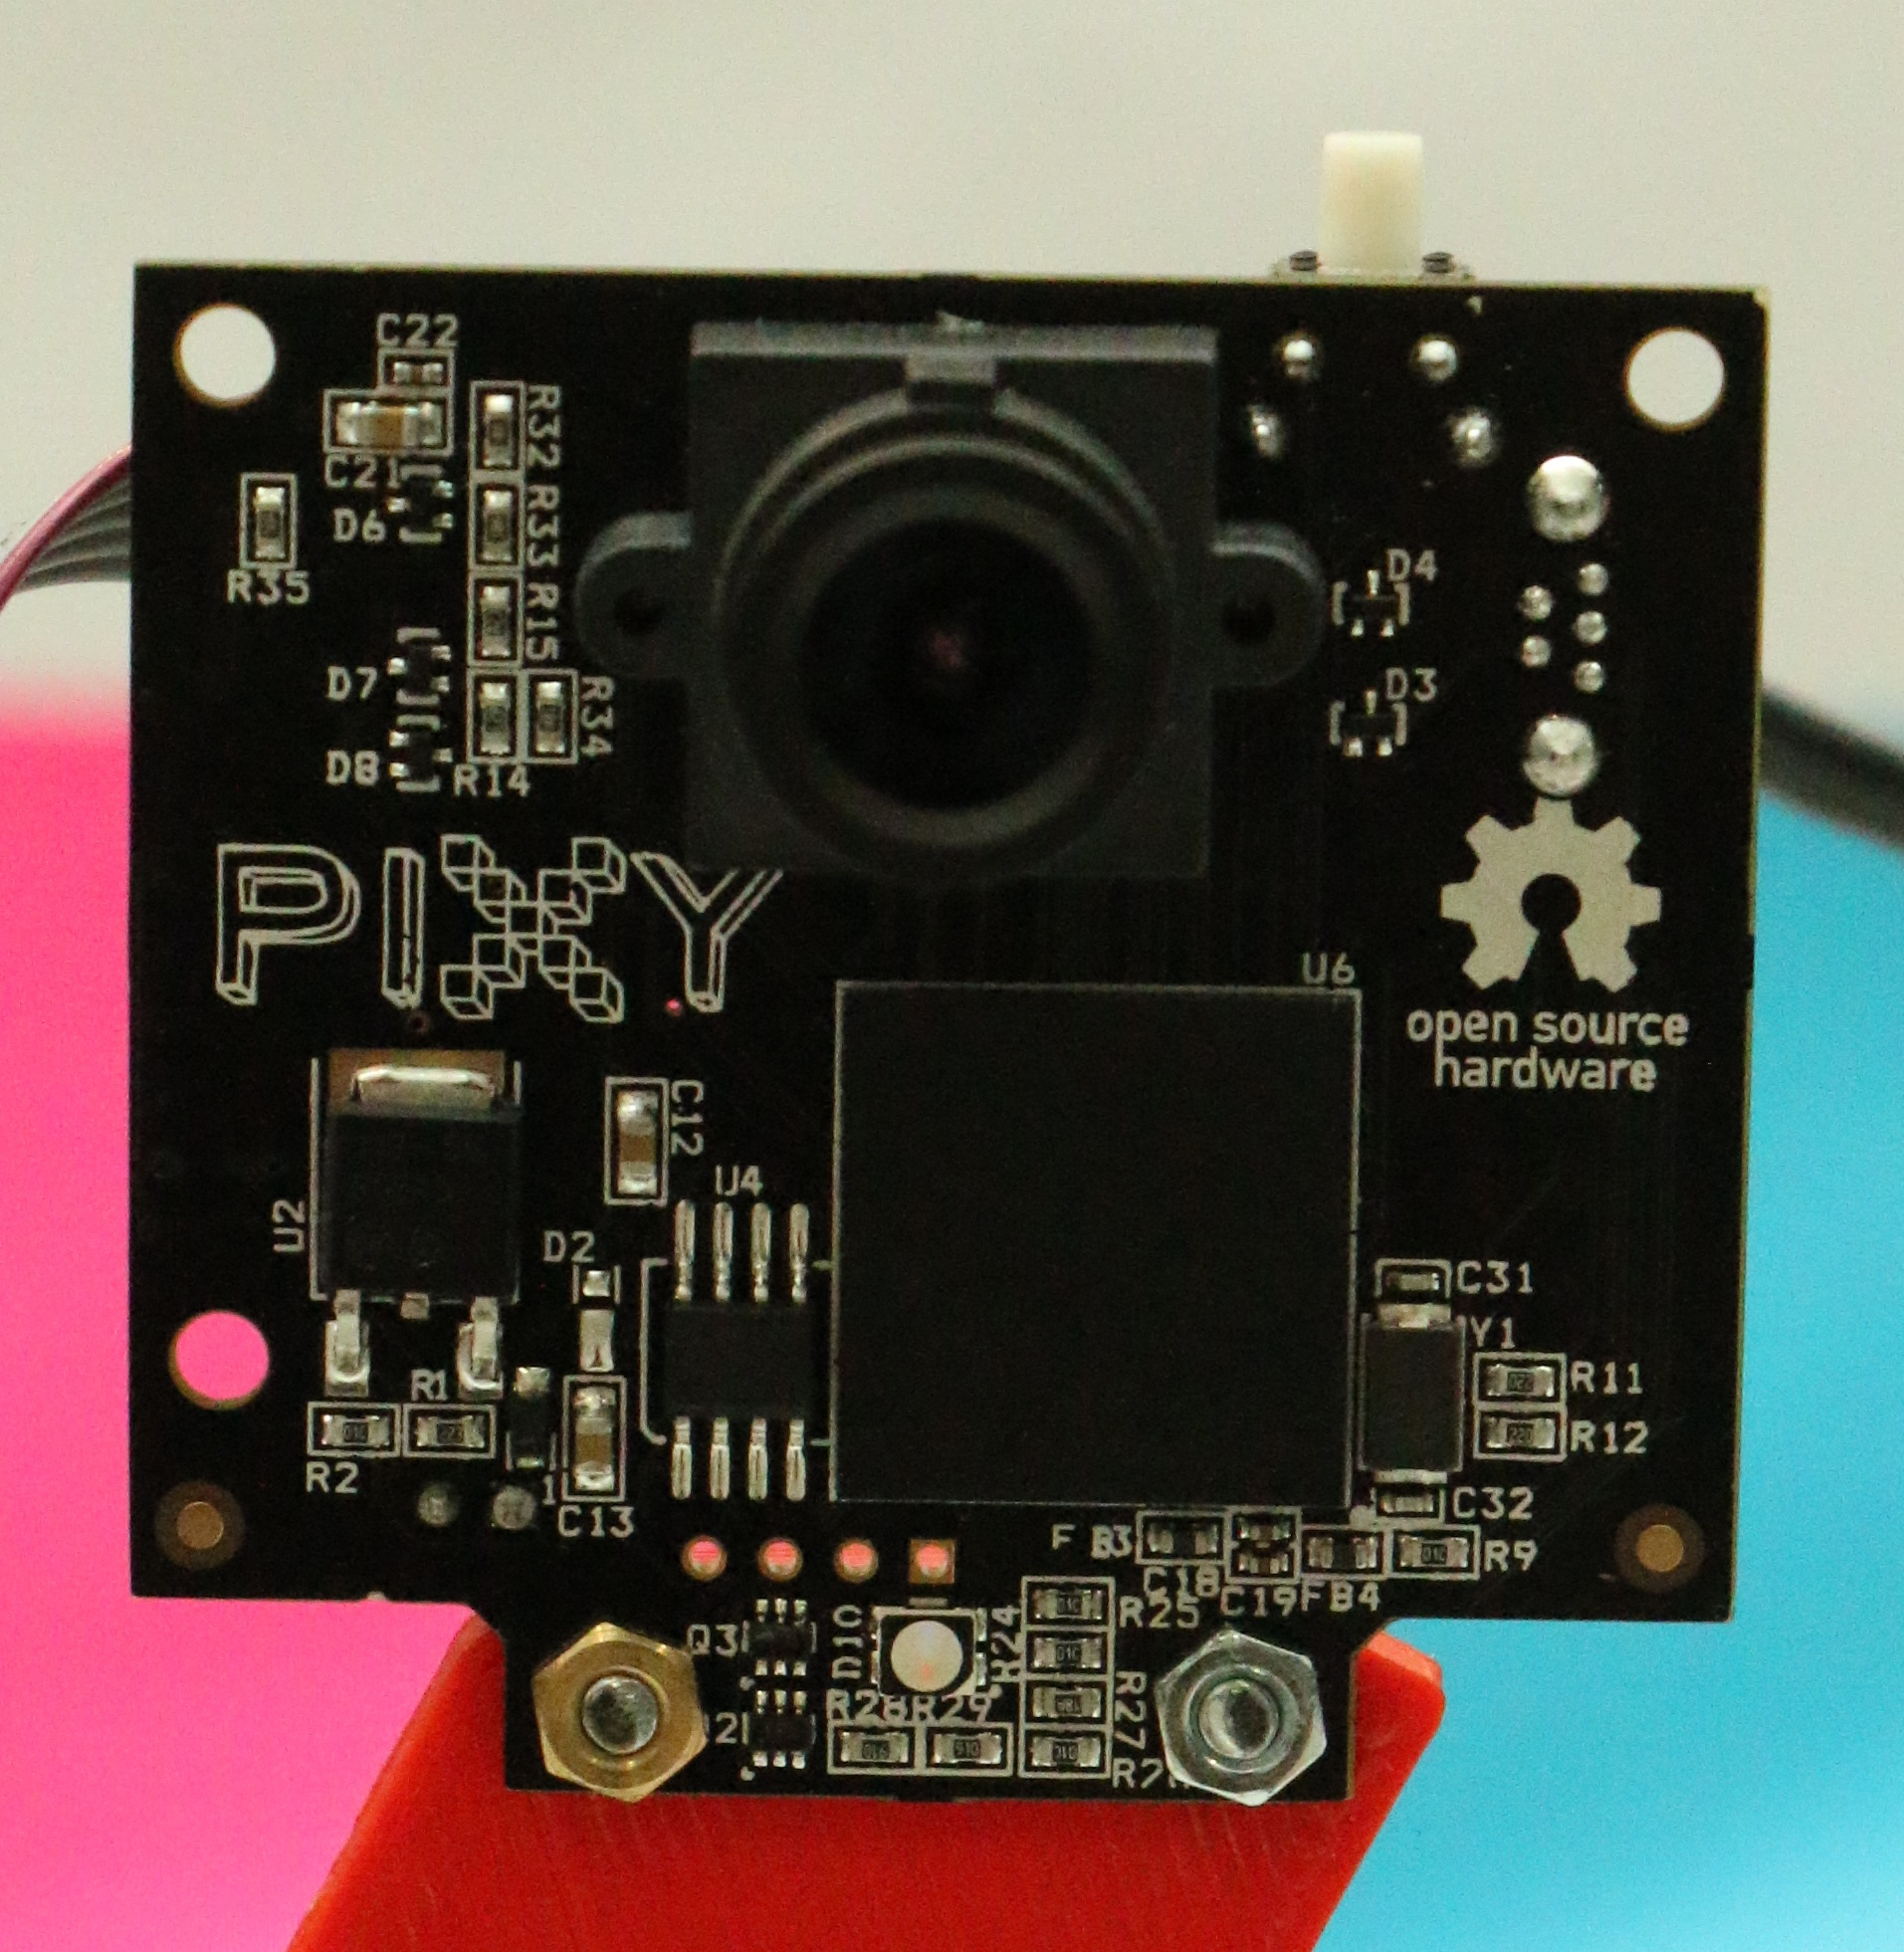
\includegraphics[width = 0.4\textwidth]{Bilder/Pixy_CMUcam5}
  \par\end{centering}
  \caption{PIXY CMUcam5}
  \label{PIXY}
\end{figure}

\begin{figure}[H]
  \begin{centering}
    \subfigure[Colorcode]{
\includegraphics[width = 0.4\textwidth]{Bilder/Colorcode}}
    \subfigure[Objekt]{
\includegraphics[width = 0.4\textwidth]{Bilder/Colorcode}} %%%%%%%%%Objekt statt Colorcode
  \par\end{centering}
  \caption{Erkennbare Objekttypen}
  \label{PIXY_Objekte}
\end{figure}

  \subsection{Technische Planung}
    \subsubsection{Mögliche Verfahren zur Positionserkennung}
    Hier muss grundsätzlich zwischen zwei Messmethoden unterschieden werden:
    \begin{itemize}
      \item \textbf{Absolute Positionsmessung}\\
      Hier wird die Postion von einem gleichbleibenden Punkt aus gemessen. Dabei ist ein konstanter Referenzpunkt wichtig. Verändert sich dieser oder kann die Distanz nicht genau gemessen werden ist die Messung unbrauchbar.

      Für eine absolute Positionsmessung bieten sich diverse Triangulationsverfahren an, diese sind ausgesprochen rechenaufwändig und benötigen meist eine sehr genaue Laufzeitmessung. Für die Triangulation können die unterschiedlichsten Signale verwendet werden, am gängigsten sind jedoch jene die mit elektromagnetischen Wellen arbeiten, \zB WLAN, Bluetooth. Dies bedeutet, dass sich die Signale mit Lichtgeschwindigkeit ausbreiten.

      Bei einer Messung derart schneller Signale muss ein hoher Aufwand betrieben werden um eine Messgenauigkeit von einigen cm zu erzielen. Eine weitere Herausforderung sind Mauern \bzw Hindernisse. Hier muss ständig berücksichtigt werden wo ein Objekt steht und ob der geplante Weg überhaupt frei ist.
      \item \textbf{Relative Positionsmessung}\\
      Hier wird die Position von einem wechselnden Punkt aus gemessen. Um hier eine Positionierung im Raum ermöglichen zu können, ist es erforderlich immer zu einem bestimmten Punkt zu messen. Ein Wechsel dieses Punktes ist jedoch möglich, deshalb muss auch die Position der Punkte im Raum bekannt sein. Ist die Zielposition im Raum bekannt kann zu dieser hin navigiert werden. Auch hier muss wie bei einer absoluten Positionsmessung auf Hindernisse geachtet werden.

      Die zweite Alternative ist, dass eine bestimmte Route bekannt ist und sich das zu positionierende Objekt nur in einem bestimmten Bereich um diese Route bewegt. Wird bei der Positionierung der Route bereits auf Hindernisse geachtet müssen diese im Anschluss nicht mehr zwingend beachtet werden.
    \end{itemize}

  \subsection{Umsetzung}
  Durch die PIXY CMUcam5 lässt sich eine relative Positionsmessung vergleichsweise einfach verwirklichen. Werden ein oder mehrere Objekte erkannt wird eine bestimmte Nummer (abhängig von der Farbe) sowie die Position am Bild und die Objektgröße übermittelt. Die Kamera arbeitet dabei mit einer Bildwiederholrate von 50 Hz, es ist also alle 20 ms eine Auswertung möglich.

  Die Kamera wird auf dem Hexacopter befestigt, mehrere Farbcodes kennzeichnen den Weg zu einem Tisch. Um an dieser Stelle eine Navigation zu erreichen wird der Hexacopter so gesteuert, dass er, abhängig von der Route, immer einen bestimmten Farbcode betrachtet, ist er über diesem sucht er den nächsten.

    \subsubsection{SPI Schnittstelle}
    Als Schnittstelle für die Kommunikation mit der Kamera wird eine SPI-Schnittstelle verwendet. Die Kamera selbst unterstützt unter anderem die seriellen Schnittstellen UART, I2C und SPI. Außerdem werden noch ein analoger und digitaler Output unterstütz, diese sind jedoch vergleichsweise beschränkt, da keine näheren Informationen zu dem Objekt übermittelt werden können sondern nur die Position \bzw ob überhaupt ein Objekt erkannt wurde.

    Die SPI-Schnittstelle ist bei der Kamera besonders ausfallsicher. Hier wird ein Synchronisationsbyte gefordert, wird dieses nicht erkannt, \zB aufgrund eines Fehlers in der Datenübertragung, schickt die Kamera keine Daten.

    \paragraph{Überprüfen der SPI-Schnitstelle}
    Um zu überprüfen ob die SPI-Schnittstelle auch korrekt arbeitet wird bei der ersten Inbetriebnahme der Output überprüft. Hierzu wird der Zustand der 3 Leitungen mit einem Oszilloskop betrachtet.
    \begin{itemize}
      \item \textcolor{blue}{Taktleitung}
      \item \textcolor{red}{Dateneingang (PIC)}
      \item \textcolor{green}{Datenausgang (PIC)}
    \end{itemize}

    \begin{figure}[tbh]
      \begin{centering}
        \subfigure[Großer Zeitbereich]{\includegraphics[width = 0.49\textwidth]{Bilder/SPI_gross}}
        \subfigure[Kleiner Zeitbereich]{\includegraphics[width = 0.49\textwidth]{Bilder/SPI_klein}}
      \par\end{centering}
      \caption{Ausgang der SPI Schnittstelle}
      \label{SPI-Ausgang}
    \end{figure}

    Der Wert mit dem diese Überprüfung durchgeführt wird sollte möglichst variabel sein, hier wird 0xAA (1010 1010) verwendet. Wird dieser Wert nicht variabel angenommen kann es dazu kommen, dass fälschlicher Weise angenommen wird, dass die Übertragung korrekt ist.
    Der Dateneingang des PIC, respektive der Ausgang der Kamera, zeigt eine deutliche Störung durch die Taktleitung an.

    \subsubsection{Erkennen und Auswerten eines Bildes}
    Die Kamera schickt der Reihe nach die einzelnen Daten eines Objekts. Darunter ist auch eine Startbedingung die ein neues Bild markiert. Mit den diversen Informationen zum Objekt ergeben sich folgende Daten:
    \begin{itemize}
      \item Neues Bild 0xAA55
      \item Objekt 0xAA55 oder Farbcode 0xAA56
      \item Checksum
      \item Objektnummer
      \item X-Position
      \item Y-Position
      \item Breite
      \item Höhe
      \item Drehwinkel, nur bei Farbcodes
    \end{itemize}
    Dabei ist die Objektnummer von den im Objekt oder Farbcode vorkommenden Farben abhängig, zusätzlich ist zu beachten, dass sie oktal dargestellt wird. Ein übermittelter Wert von dezimal 10, also oktal 12, bedeutet, dass die Farben 1 und 2 erkannt wurden.

    Will man nun ein neues Bild finden muss man so lange nach 0xAA55 suchen bis man diese Daten gesendet bekommt. Anschließend gilt es noch festzustellen ob man einen Farbcode oder ein Objekt betrachtet, es muss also direkt darauf 0xAA56 oder nochmals 0xAA55 erkannt werden. Ist dies nicht der Fall, wurde kein neues Bild erkannt und man betrachtet ein normales Objekt.

    Betrachtet man nun die bis zum Erkennen eines neuen Bildes gesendeten Daten als gegenstandslos ergibt sich eine vergleichsweise einfache Schleife um ein Bild zu erkennen.

    \lstset{language = c}
    \begin{lstlisting}
while(frame == 0) {
  w = ExchangeSpiWord(PIXY_SYNC, DUMMY);
  if(lw == PIXY_FRAME_OBJ && w == PIXY_FRAME_OBJ) {
    frame = 1;
    obj_type = 0;
    a_color[c_obj].type = PIXY_FRAME_OBJ;
  } else if(lw == PIXY_FRAME_OBJ && w == PIXY_COLORCODE) {
    frame = 1;
    obj_type = 1;
    a_color[c_obj].type = PIXY_COLORCODE;
  } else if(w == 0 && lw == 0){
    frame = 0;
  }
  lw = w;
  c++;
  if(c > 254) {
    return 0;	//****Error, end of function
  }
}
    \end{lstlisting}
    Um nicht ewig in dieser Schleife fest zu hängen, wenn kein Bild erkannt wird und einen Fehler auslösen zu können wird die gesamte Funktion der Bildauswertung nach 255 Versuchen verlassen.

    Die weiteren Werte eines Objekts werden der Reihe nach in einer Structur abgespeichert, hier ist nichts besonderes mehr zu beachten.

  \subsection{Herausforderungen und Lösungen}

%%%%%%%%%%%%%%%%%%%%%%%%%%%%%%%%%%%%%%%%%%%%%%%%%%%%%%%%%%%%%%%%%%%%%%%%%%%%%%%
\section{Ultraschall}

  \subsection{Technische Planung}

  \subsection{Umsetzung}

    \subsubsection{Bestimmen der Flughöhe}

  \subsection{Herausforderungen und Lösungen}

\chapter{Aktoren}
\renewcommand{\kapitelautor}{Autor: Lucas Ullrich}

%%%%%%%%%%%%%%%%%%%%%%%%%%%%%%%%%%%%%%%%%%%%%%%%%%%%%%%%%%%%%%%%%%%%%%%%%%%%%%%
\section{Propeller, A E T und R}

  \subsection{Technische Planung}

  \subsection{Umsetzung}

  \subsection{Herausforderungen und Lösungen}
